\input{fixos/pacotes}
\input{fixos/comandos}
\input{fixos/novosComandos}

% Dados pessoais
\autor{Álvaro Fernando Matos de Souza}
\curso{Engenharia de Software}

% Dados do trabalho
\titulo{Análise Exploratória do Projeto Mezuro: uma Proposta de Evoluç\~ao da
Apresentação das Métricas de Código-fonte}
\data{2016}
\palavraChaveUm{Engenharia de Software}
\palavraChaveDois{Visualização de Software}
\palavraChaveTres{Métricas de código-fonte}
\palavraChaveQuatro{Evolução de Software}

% Dados da orientacao
\orientador{Prof. Dr. Paulo Roberto Miranda Meirelles}
\coorientador{Rafael Reggiani Manzo}

% Dados para a ficha catalográfica
\cdu{}

% Dados da aprovação do trabalho
\dataDaAprovacao{Dezembro de 2015}
\membroConvidadoUm{Rafael Messias Martins}
\membroConvidadoDois{Titulação e Nome do Professor Convidado 02}

% Dados pessoais
\autor{Álvaro Fernando Matos de Souza}
\curso{Engenharia de Software}

% Dados do trabalho
\titulo{Análise Exploratória do Projeto Mezuro: uma Proposta de Evoluç\~ao da
Apresentação das Métricas de Código-fonte}
\data{2016}
\palavraChaveUm{Engenharia de Software}
\palavraChaveDois{Visualização de Software}
\palavraChaveTres{Métricas de código-fonte}
\palavraChaveQuatro{Evolução de Software}

% Dados da orientacao
\orientador{Prof. Dr. Paulo Roberto Miranda Meirelles}
\coorientador{Rafael Reggiani Manzo}

% Dados para a ficha catalográfica
\cdu{}

% Dados da aprovação do trabalho
\dataDaAprovacao{Dezembro de 2015}
\membroConvidadoUm{Rafael Messias Martins}
\membroConvidadoDois{Titulação e Nome do Professor Convidado 02}

\input{fixos/setup}

\begin{document}

\frenchspacing
\imprimircapa
\imprimirfolhaderosto*

\input{fixos/fichaCatalografica}
\input{editaveis/errata}
\input{fixos/folhaDeAprovacao}
\begin{agradecimentos}

Agradeço a Deus pelos dons e capacidades cognitivas. Ao meu orientador, Paulo
Roberto Miranda Meirelles por já em nossos primeiros encontros em sala de aula,
em 2013 (primeiro ano como professor da UnB-FGA), na disciplina de Técnicas de
Programação, enxergar em mim algum potencial e confiar desde o início a
participação em projetos que cito hoje como as minhas primeiras experiências
profissionais, que certamente me ajudaram e ainda irão produzir frutos. Agradeço
aos amigos Carlos Coêlho, Fagner Rodrigues, Leandro Alves, João Paulo Alves e
Yeltsin Suares que foram de fundamental apoio para minha formação, iniciaram o
curso comigo e até hoje estão próximos. Aos mestrandos Diego Araújo e Rafael
Manzo, pois sem as instruções e disponibilidade deles este trabalho de conclusão
não seria realizado. Aos vários colegas de classe que compartilharam os mais
diversos momentos de alegrias e frustrações, e que amigavelmente me apelidaram de
“Jesus”! São muitos os nomes, mas se em algum momento tivemos que virar uma
noite finalizando algum trabalho/projeto/estudo, saiba que foi uma honra e que
agradeço o compartilhamento mútuo de conhecimento e risadas. Aos colegas,
professores e profissionais seniores do Laboratório Avançado de Produção,
Pesquisa \& Inovação em Software (LAPPIS) pelas várias horas empenhadas em
construir software sem nos precipitarmos, tendo calma cinco vezes e não sendo
egoístas. Agradeço aos meus pais, José Fernando e Edna, e às minhas irmãs,
Angélica e Heloísa, que me apoiaram e me sustentaram incondicionalmente, e por
serem os únicos que me viram deitar mesmo no chão para tentar relaxar no final
de semestres difíceis. Agradecimento especial à minha namorada, Nicole Pachêco,
que foi a peça fundamental para a minha mudança na vida acadêmica, pela
compreensão e carinho, e por ter sido minha fiel espectadora nos ensaios para a
defesa deste trabalho e também fiel revisora gramatical (manja muito das
letras!). Por fim, aproveito para reforçar um agradecimento especial para minha
mãe, Edna Matos de Souza, e dedicar à ela este trabalho, pois sem ela não
conseguiria caminhar (figurativamente e literalmente) e com certeza não me
tornaria Engenheiro de Software. Muito obrigado!

\end{agradecimentos}

\begin{epigrafe}
    \vspace*{\fill}
	\begin{flushright}

		\textit{``O temor do SENHOR é o princípio da sabedoria, \\
		e o conhecimento do Santo é prudência.''\\
		(Bíblia Sagrada, Provérbios 9, 10)}
	\end{flushright}
\end{epigrafe}

\begin{resumo}
 O Mezuro é uma plataforma web livre de avaliação de código-fonte.
 As métricas são expostas por meio de números e grupos de leituras.
 O objetivo deste trabalho é evoluir a visualização das métricas de
 código dos softwares analisados pelo Mezuro. Como contribuição científica,
 ou atividade de pesquisa, será realizado o estudo das possíveis técnicas
 de visualização de software e suas combinações com as métricas de
 código-fonte. E como atividade tecnológica será proposto a visualização
 de um conjunto de métricas determinado, evolução das configurações de
 métrica do Mezuro e será proposto a contribuição aos mantenedores desta
 plataforma.

 \vspace{\onelineskip}
    
 \noindent
 \textbf{Palavras-chaves}: Engenaria de Software. Visualização de Software.
 Métricas de código-fonte. Evolução de Software.
\end{resumo}

\begin{resumo}[Abstract]
 \begin{otherlanguage*}{english}
   The Mezuro is a free Web platform evaluation of source code. The metrics are
   exposed through numbers and readings groups. The objective of this work is
   to evolve the visualization of metrics code of the software analyzed by
   Mezuro.
   The following contributions are planned: validation of metrics settings of
   the Mezuro and software visualization specification.
   As a scientific contribution, or research activity, will be done the analysis
   of the projects available on the Portal of the Brazilian Public Software
   (SPB).
   And the study of possible software visualization techniques applied to
   Mezuro.

   \vspace{\onelineskip}

   \noindent
   \textbf{Key-words}: Software Engineering. Mezuro. Software visualization.
   Metrics for source code. Software Evolution. Brazilian Public Software.
 \end{otherlanguage*}
\end{resumo}

\input{fixos/listasAutomaticas}
\begin{siglas}
  \item[VS] Visualização de Software
\end{siglas}

\input{fixos/indiceAutomatico}

\textual

\chapter{Introdução}

% TODO: SUPER TAREFA! Organizar imagens/figuras antes dos textos que as explicam

A chamada ``crise do software'' \cite{arthur1985measuring} foi a grande
responsável pela necessidade de averiguação e evolução da qualidade do produto
da engenharia de software. Os requisitos que definem a qualidade de um sistema
e também estão envolvidos com a sua complexidade são
\cite{behkamal2009customizing}: execução correta das funcionalidades previstas;
confiabilidade; usabilidade; eficiência; manutenibilidade; e portabilidade. Para
o desenvolvimento de um software, são levados em consideração aspectos como
tamanho e interação entre os diversos componentes \cite{koscianski2007qualidade},
podendo não seguir as diretrizes de qualidade da ISO 9126 de
\citeonline{behkamal2009customizing}.

Aspectos da qualidade não são claros em muitos softwares atualmente e existe
uma grande complexidade em entender o seu funcionamento. A visualização de
software pode auxiliar e ou facilitar o entendimento destes aspectos e pode
reduzir essa complexidade \cite{messias2012} \cite{benkler2006wealth}. Não
faltam dados disponíveis publicamente para auxiliar na geração desse
entendimento: código-fonte, históricos de evolução do repositório, conjuntos de
testes, relatórios de erros e suas soluções, trocas de mensagens entre membros
do projeto em listas de e-mail, artigos escritos por acadêmicos que buscam fama,
entre outros \cite{messias2012} \cite{benkler2006wealth}.

Desenvolvedores são cruciais para o sucesso de um projeto. Os valores
numéricos dos vários locais com dados disponibilizados publicamente em que é
possível coletar os dados citados no parágrafo anterior, eventualmente podem não
ter uma boa apresentação. Os dados podem ser de pouco valor, pois são numerosos
e difíceis de avaliar. Uma possível solução: visualização de informação
\cite{messias2012}. Visualização de informação é toda aquela representação
desenvolvida por computador que tem como objetivo a geração e aplicação de
conhecimento \cite{card1999readings}. Podem ser interativas ou não, e podem
influenciar analistas de dados nas tomadas de decisões e na transmissão desses
conhecimentos a partir de dados complexos \cite{card1999readings}. Um problema
da Visualização de Software (VS) é selecionar uma técnica, pois nenhuma técnica
específica funciona para todos os problemas.

O software livre apresenta certas vantagens em detrimento do software restrito.
Geralmente licenciado sob as definições da
\textit{Free Software Foundation}\footnote{\url{http://www.gnu.org/philosophy/free-sw.pt-br.html}},
ou da \textit{Open Source Initiative}\footnote{\url{https://opensource.org/docs/definition.html}},
o software livre e aberto (\textit{Free and Open Source Software} - FOSS) tem
seu código aberto e acessível ao público e garante ao programador certos
aspectos que podem simplificar o desenvolvimento de um novo software ou a
evolução de um outro onde o envolvimento é desejado, seja por questões de
melhoria, ética, personalização ou simplesmente pelo interesse pessoal
\cite{meirelles2013monitoramento}. E muitas outras características agregam
valor ao uso, desenvolvimento e estímulo às contribuições ao FOSS: o
estabelecimento de uma \textit{cultura livre}, valorizando o mérito de questões
técnicas inerentes ao desenvolvedor; reconhecimento de bons programadores
capazes de escrever bons códigos e outros programadores melhores ainda capazes de
mantê-los; reconhecimento do valor das pessoas envolvidas e interessadas, sejam
usuários finais, sejam testadores de versões instáveis do software; entre outras
características \cite{raymond1999cathedral}.

Neste trabalho, é apresentada uma análise exploratória da plataforma \textbf{livre}
Mezuro\footnote{\url{http://mezuro.org/}}, que é uma ferramenta de monitoramento
de código-fonte. Primeiramente foi-se pensado para esta análise a verificação da
necessidade de aplicação de técnicas de Visualização de Software na plataforma
Mezuro. Isso porque é estabelecido como motivação identificar os motivos do
baixo número de usuários e número de projetos no Mezuro, em comparação, por
exemplo, com o Code Climate\footnote{\url{https://codeclimate.com/}}, que foi
desenvolvido posteriormente ao Mezuro.

Para realizar a análise exploratória proposta, inicialmente foi necessário
validar uma das principais funcionalidades do Mezuro que são as configurações
para a intepretação dos valores de métricas. Isso porque, os exemplos de uso
selecionados para esta análise foram os projetos do Portal do Software
Público Brasileiro (SPB), em que estava previsto para a incorporação do Mezuro.

\section{Objetivos}

O objetivo deste trabalho é avaliação da exibição dos dados das métricas de
código-fonte, com intuito de apontar evoluções para o Mezuro deixar de ser uma
plataforma em estado ``Beta''.
%
Isto também com o objetivo de explorar todo funcionamento do Mezuro, em especial,
com foco nos coletores adicionados recentemente para projetos desenvolvidos nas
linguagens de programação PHP e Python, no contexto da avaliação dos projetos do
Portal do Software Público Brasileiro.
%
Assim gerando insumos para comparação do Mezuro com outras plataformas de
avaliação de métricas de código-fonte.

\section{Organização do Trabalho}

O trabalho está organizado da seguinte maneira: Capítulo \ref{chap:mezuro}, onde
será tratado o Mezuro como principal ferramenta, foco da análise exploratória;
Capítulo \ref{chap:visualizacao}, onde será tratada a Visualização de Software
como principal base para o referencial teórico e revisão bibliográfica do estudo
sobre VS; Capítulo \ref{chap:metodologia}, que trata da metodologia para o
desenvolvimento do mesmo; no Capítulo \ref{chap:analise_exploratoria} é
apresentada a análise exploratória de fato do Mezuro, com explicação de um dos
casos de uso; Capítulo \ref{chap:proposta}, com a proposta de melhoria para o
Mezuro; e o Capítulo \ref{chap:conclusao} com as conclusões e trabalhos futuros.

% Introdução com forte embasamento em Métodos Ágeis e FOSS, e Visualização pra apoiar
% citar PRMM, Fábio Kon... (verificar refereências do Messias)
\input{capitulos/2-visualizacao_de_software}
% TODO: INICIAR COM O CAPÍTULO 2 SOBRE VISUALIZAÇÃO
% capitulo 2 - visualização - com seção de métricas
% msg pro leitor: explicar visu, oq ele precisa saber para ler o meu TCC
\chapter{Metodologia}

\section{Objetivos}

O objetivo deste capítulo é apresentar a metodologia utilizada para a
realização da pesquisa e contribuição tecnológica. A principal questão
a ser respondida é: como a visualização de software pode auxiliar na
interpretação das métricas coletas e calculadas por ferramentas de análise
de código?

Considerando esta questão, é importante ressaltar que existem incontáveis
destas ferramentas. Porém estas analisam apenas aspectos mui específicos
do software, e falham (algumas delas) em demostrar ao engenheiro de
qualidade a interpretação dos dados analisados \cite{deissenboeck2011}.

Neste trabalho serão unidas determinadas métricas (TODO: definir quais
métricas), para gerar uma ou várias visualizações que auxiliem o usuário
do Mezuro a ter uma melhor interpretação do resultado gerado por esta
ferramenta.

Como exemplo dessa união e para a construção da prova de conceito
(TODO: é esse mesmo o nome?), é proposto utilizar-se da decisão dos
colegas Renan Costa Filgueiras e Vinícius Vieira Meneses: foram escolhidas
três métricas para a configuração da visualização em radar: \textit{number
of methods} (código: npm), \textit{number of public methods} (código nom)
e \textit{total number of modules} (código: total\_modules); e a decisão
de utilizar a biblioteca Javascript \textit{D3.js - Data-Driven Documents}.
(TODO: adicionar referência)

\section{Trabalhos Relacionados}

\section{Questão Problema e Hipóteses}

Reforçando a questão problema (QP), foram levantadas estas outras abaixo:

\begin{itemize}
  \item QP1 - Como a visualização de software pode auxiliar na
  interpretação das métricas coletadas e calculadas pelo Mezuro?
  \item QP2 - Quais técnicas de visualização que melhor se adequam ao
  contexto do Mezuro, possibilitando a aplicação em qualquer contexto de
  configuração?
  \item QP3 - Como representar as diferentes perspectivas sobre o processo
  de desenvolvimento e o produto de software?
\end{itemize}

As hipóteses são:

\begin{itemize}
  \item H1 - Não haverá uma visualização única para todas as métricas.
  \item H2 - Algumas métricas poderão ser apresentadas de uma forma combinada
  em uma única represetação/visualização.
\end{itemize}

% TODO: elaborar e documentar as hipótees

\section{O Mezuro}

O projeto Mezuro é uma ferramenta para extração, análise e interpretação de
métricas de código-fonte. De uma forma geral, ele é dividido em duas partes:
para o processamento e para o cálculo é utilizado o Kalibro, que é um
\textit{webservice}; e o Prezento para a interface gráfica (uma aplicação
\textit{Web}) \cite{meirellesCibse2015}. Sob a licença
\textit{Affero General Public License version 3} (AGPLv3), o Mezuro permite que
o usuário crie, salve e edite ``configurações'' que são um conjunto de
métricas escolhidas por este e um ``grupo de leitura'' para provimento de uma
interface gráfica de um conjunto de leitura que tenha algum sentido quando
agrupadas, por exemplo: com a pontuação x, a métrica terá o ``rótulo'' ``BOM'' e
será atribuído à ela a cor amarela; com a pontuação x+2, a métrica terá o 
``rótulo'' ``ÓTIMO'' e estará com a cor verde. As cores são para destacar a
interpretação e são definidas com valores hexadecimal \cite{camarinhaOSS2015}.

O Kalibro, citado no parágrafo anterior, foi inicialmente escrito em Java para
compor uma das ferramentas do projeto QualiPSo (\textit{Quality Platform for
Open Source Software}). Já possuía maioria das funcionalidades presentes na
versão atual do Mezuro. Uma delas, bastante prática, é a de fornecer apenas o
URL do código compactado em arquivo ZIP ou TARBALL, ou o link para as
aplicações de controle de versão em SVN ou GIT, mais a escolha de uma
configuração, para iniciar a análise \cite{camarinhaOSS2015}. Em 2013 o Mezuro
passou a ser reescrito em Ruby, com objetivo de manter na mesma tecnologia as
camadas da arquitetura. Mudança justificada também pela necessidade do
processamento dos cálculos e da análise. A carga de requisições, mais a
quantidade de núcleos que o servidor possuía, faziam com que a versão original
do Kalibro ficasse debilitado em seu fluxo de execuções. Outra vantagem dessa
reescrita é a facilidade com que novos contribuidores puderam/poderão entender
todo o funcionamento dessa parte do Mezuro. Algumas funcionalidades foram
eliminadas por serem consideradas não essenciais. E grande parte da primeira
versão do Kalibro está presente na gema
kalibro\_gem\footnote{\url{https://rubygems.org/gems/kalibro_gem}}
\cite{meirellesCibse2015}.

% TODO: a gem kalibro\_gem e a kalibro\_client são a mesma coisa? A kalibro\_gem
% foi descontinuada?)

% Sobre o Prezento

O Kalibro foi construído, nos primórdios, como um plugin da rede social
Noosfero. Com a decisão de reescrevê-lo em Ruby, a antiga interface gráfica,
que era aproveitada do Noosfero, foi também reescrita nesta
tecnologia. O Prezento, desenvolvido utilizando o \textit{framework} para
desenvolvimento de aplicações \textit{Web}
Ruby on Rails\footnote{\url{http://guides.rubyonrails.org/getting_started.html}},
é a redesenha e atual interface.

% Sobre a arquitetura do Mezuro

% (Eu preciso falar do QualiPSo?  Não!)

O projeto QualiPSo, iniciado em meados de 2007, tinha como objetivo aprimorar
as práticas de desenvolvimento aberto à época para atingir o reconhecimento e
confiabilidade que o FOSS possui hoje \cite{messias2012}.

\subsection{Arquitetura e principais funcionalidades do Mezuro}

Com a reescrita, a arquitetura do Mezuro foi dividida em três serviços:

\begin{itemize}
  \item Prezento: para a interface gráfica do usuário
  \item Kalibro Processor: para a análise do código
  \item Kalibro Configuratios: para o gerenciamento das configurações
\end{itemize}

A decisão de dividir o Kalibro em serviços separados foi tomada para deixar
cada um deles com menos responsabilidades, facilitando a manutenção e evolução
\cite{camarinhaOSS2015}. E a comunicação entre estes serviços é feita através
do Kalibro Client: um quarto software também escrito em Ruby, mantendo a
escolha de centralização em uma única tecnologia. E para simplificar a
implementação, também foi decidido que a comunicação entre os serviços seria
RESTful.

As figuras a seguir demonstram como a comunicação funciona, um diagrama UML de
sequência do processo de criação de uma configuração chegando ao estágio em que
são expostos os resultados finais de uma análise após a reescrita da interface
gráfica, e outra que demonstra o estado atual do projeto.

% TODO: Alterar essa primeira imagem para representação da atual arquitetura

\begin{figure}[!htb]
	\centering
	\label{mezuroNoosferoArch}
		\includegraphics[keepaspectratio=true,scale=0.5]{figuras/mezuroCloudArch.eps}
	\caption{Arquitetura do Mezuro \cite{camarinhaOSS2015}}
\end{figure}

\begin{figure}[!htb]
	\centering
	\label{prevProcessingSeqDiag}
		\includegraphics[keepaspectratio=true,scale=0.7]{figuras/prevProcessingSeqDiag.eps}
	\caption{Arquitetura do sistema ao fim da reescrita da interface gráfica
	\cite{meirellesCibse2015}}
\end{figure}

\begin{figure}[!htb]
	\centering
	\label{processingSeqDiag}
		\includegraphics[keepaspectratio=true,scale=0.5]{figuras/processingSeqDiag.eps}
	\caption{Arquitetura do sistema ao fim da reestruturação do Kalibro
	\cite{meirellesCibse2015}}
\end{figure}

\newpage

Segundo \citeonline{camarinhaOSS2015}, as principais ``funcionalidades podem ser
divididas em dois grupos:

\begin{itemize}
  \item Projeto
    \begin{itemize}
    \item \textit{Download} do código-fonte a partir de repositórios (Git,
    Subversion, Bazaar etc) ou via arquivo compactado;
        \item Escolha da periodicidade do processamento do código (1 dia, 2 dias,
        semanal, quinzenal e mensal);
        \item Escolha de qual configuração de métricas cada repositório irá
        utilizar;
        \item Nota de cada métrica da configuração para cada arquivo do
        repositório;
        \item Análise gráfica de cada arquivo do repositório por meio de um
        gráfico de pontos com notas ao longo do tempo;
        \item Resultados públicos e acessíveis à comunidade.
    \end{itemize}
    \item Configuração
    \begin{itemize}
    \item Criação de configuração e a possibilidade de clonagem;
        \item Estatísticas sobre as configurações mais populares dentro da
        comunidade;
        \item Criação de intervalos qualitativos associados aos valores das
        métricas;
        \item Criação de grupos de leitura para a interpretação textual dos
        resultados das métricas;
        \item Combinações de métricas nativas para criação de análises compostas
        e mais complexas.''
    \end{itemize}
\end{itemize}
''
% TODO: consertar estas aspas na citação direta
% TODO: posso fazer esta citação direta?

\newpage

\section{A Decisão de utilizar o Mezruo}

Para este trabalho de conclusão de curso a ferramenta de de análise de código
fonte escolhida foi o Mezuro pois: o aluno já participou da evolução de parte
de algumas funcionalidades; a ferramenta proporciona ao usuário a análise
periódica do projeto, o que atende ao desejado como contribuição tecnológica
das visualizações geradas serem demonstradas ao longo do tempo; por ser uma
plataforma livre; fácil contato com os mantenedores; e por esta plataforma
estar sempre utilizar as últimas versões estáveis do Ruby e do Rails, ou seja,
por utilizar o que há de mais atual nestas tecnologias.

% TODO: deve adicionar mais motivações? Quais? Sei que devo, porém estou sem ideias

É importante ressaltar que outras ferramentas de análise de código poderão ser
utilizadas para geração da visualização proposta neste trabalho. Pois o fluxo
básico de execução permitirá tal geração, a saber: análise pela ferramenta,
dados exportados de forma determinada para anteder a leitura da biblioteca JS,
geração da visualização em um terceiro serviço local ou remoto.

E o ideal é que este trabalho sirva como base para a criação de futuras
visualizações para o Mezuro em si.

\section{Proposta de Evolução da Visualização}

\section{Seleção das Métricas}

% TODO: selecionar métricas com certo nível de similaridade.
% TODO: citar aqui talvez Michelle Lanza e R Marinescu - software metrics

% capitulo 3 - metodologias, vem o mezuro
\chapter{Resultados Preliminares}

\section{Mezuro: Prezento}

% TODO: falar sobre o Prezento, pois será a camada em que irei trabalhar

\section{D3 - Data-Driven Documents}

\section{Implementação - Prova de Conceito}

\section{Exemplo de Uso}

% TODO: escolher 3 projetos para serem alvo
% TODO: escolher quais métricas

\section{Visualização - Gráfico Radar}

\chapter[Conclusão]{Conclusão}

\section{Seção 1}

\section{Seção 2}

\bookmarksetup{startatroot}

\postextual

\bibliography{bibliografia}
\begin{apendicesenv}

\partapendices

\chapter{Primeiro Apêndice}
\label{chap:apendiceA}

Resultado completo da pesquisa realizada.

\begin{figure}[!htb]
	\centering
    \includegraphics[keepaspectratio=true,scale=0.35]
    {figuras/res1.eps}
  \caption{Respostas para qual visualização foi considerada de melhor
  interpretação}
  \label{fig:res1}
\end{figure}

\begin{figure}[!htb]
	\centering
    \includegraphics[keepaspectratio=true,scale=0.35]
    {figuras/res2.eps}
  \caption{Respostas para qual visualização possuia maior clareza na
  identificação dos pontos críticos}
  \label{fig:res2}
\end{figure}

Comentários, críticas e sugestões (6 respostas). Todas as respostas foram
anônimas:

\textit{``Se o método de Node With Interations, do Lars Kotthoff, começasse com
alguns nós expandidos, ele seria o melhor (na minha opinião) de longe. Como
isso não está ocorrendo, ele ainda continua melhor (na minha opinião), mas os
outros dois são mais claros para se ver o resultado final a respeito das
métricas.''}

\textit{``O primeiro eu não entendi como funciona, se entendesse deve ser legal. O
segundo me deu dor de cabeça só de abrir a imagem e é ruim ficar virando a
cabeça e espremendo os olhos pra enxergar (tenho miopia)  O terceiro é legal
porque mostra tudo separadinho mas é um saco ter que clicar mil vezes pra ver
tudo.''}

\textit{``Poderia colocar uma opção de visualização: Node Link With Interation
by Lars Kotthoff de vizsualizar tudo de uma vez, um expand all.}

\textit{``Para a forma de visualização do Node Link With Interation by Lars
Kotthoff (adapted) seria interessante ter um aspecto de botão para a pessoa
saber que o elemento é para ser clicado.''}

\textit{``A nível de entendimento e clareza a visualização em Node Link With
Interation é a melhor, no entanto a que se apresenta de forma mais bonita é a
Node Link Tree, embora não seja tão intuitiva quanto a anterior. Além disso, a
No Link With Interation parece ter demonstrado ter capturado melhor as
necessidades, conforme a leitura das métricas, na medida em que visualmente
aponta mais valores em VERMELHO que a opção Node Link Tree. A Random Radar
Chart não evidencia valores. Não há uma escala, o que dificulta
o entendimento da gravidade da situação de uma determinada métrica.''}

\textit{``Node Link Tree by Mike Bostock é a melhor, mas para ser o mais claro é
preciso trabalhar melhor com as cores usando os valores agregados de métricas.
Coloque cores em todos os nós do grafo de acordo com o grade.''}

\end{apendicesenv}

\begin{anexosenv}

\partanexos

\chapter{Primeiro Anexo}
\label{chap:anexoA}

Resultado completo da pesquisa realizada.

\begin{figure}[!htb]
	\centering
    \includegraphics[keepaspectratio=true,scale=0.35]
    {figuras/res1.eps}
  \caption{Respostas para qual visualização foi considerada de melhor
  interpretação}
  \label{fig:res1}
\end{figure}

\begin{figure}[!htb]
	\centering
    \includegraphics[keepaspectratio=true,scale=0.35]
    {figuras/res2.eps}
  \caption{Respostas para qual visualização possuia maior clareza na
  identificação dos pontos críticos}
  \label{fig:res2}
\end{figure}

Comentários, críticas e sugestões (6 respostas). Todas as respostas foram
anônimas:

\textit{"Se o método de Node With Interations, do Lars Kotthoff, começasse com
alguns nós expandidos, ele seria o melhor (na minha opinião) de longe. Como
isso não está ocorrendo, ele ainda continua melhor (na minha opinião), mas os
outros dois são mais claros para se ver o resultado final a respeito das
métricas."}

\textit{"O primeiro eu não entendi como funciona, se entendesse deve ser legal. O
segundo me deu dor de cabeça só de abrir a imagem e é ruim ficar virando a
cabeça e espremendo os olhos pra enxergar (tenho miopia)  O terceiro é legal
porque mostra tudo separadinho mas é um saco ter que clicar mil vezes pra ver
tudo."}

\textit{"Poderia colocar uma opção de visualização: Node Link With Interation
by Lars Kotthoff de vizsualizar tudo de uma vez, um expand all.}

\textit{"Para a forma de visualização do Node Link With Interation by Lars
Kotthoff (adapted) seria interessante ter um aspecto de botão para a pessoa
saber que o elemento é para ser clicado."}

\textit{"A nível de entendimento e clareza a visualização em Node Link With
Interation é a melhor, no entanto a que se apresenta de forma mais bonita é a
Node Link Tree, embora não seja tão intuitiva quanto a anterior. Além disso, a
No Link With Interation parece ter demonstrado ter capturado melhor as
necessidades, conforme a leitura das métricas, na medida em que visualmente
aponta mais valores em VERMELHO que a opção Node Link Tree. A Random Radar
Chart não evidencia valores. Não há uma escala, o que dificulta
o entendimento da gravidade da situação de uma determinada métrica."}

\textit{"Node Link Tree by Mike Bostock é a melhor, mas para ser o mais claro é
preciso trabalhar melhor com as cores usando os valores agregados de métricas.
Coloque cores em todos os nós do grafo de acordo com o grade."}


\chapter{Segundo Anexo}
\label{chap:anexoB}

As cores de fundo das colunas "Link Mezuro" e "Link CodeClimate", represetam o
resultado das análises realizadas por estas ferramentas. Se verde, a análise foi
realizada com sucesso. Se amarelo, a análise foi concluída, porém as métricas
não foram carregadas. E quando o fundo é vermelho, a análise não obteve êxito.

% TODO: organizar estas tabelas com as mudanças de ? --> indefinido
% - e outras difinições de linguagens

\begin{figure}[!htb]
	\centering
    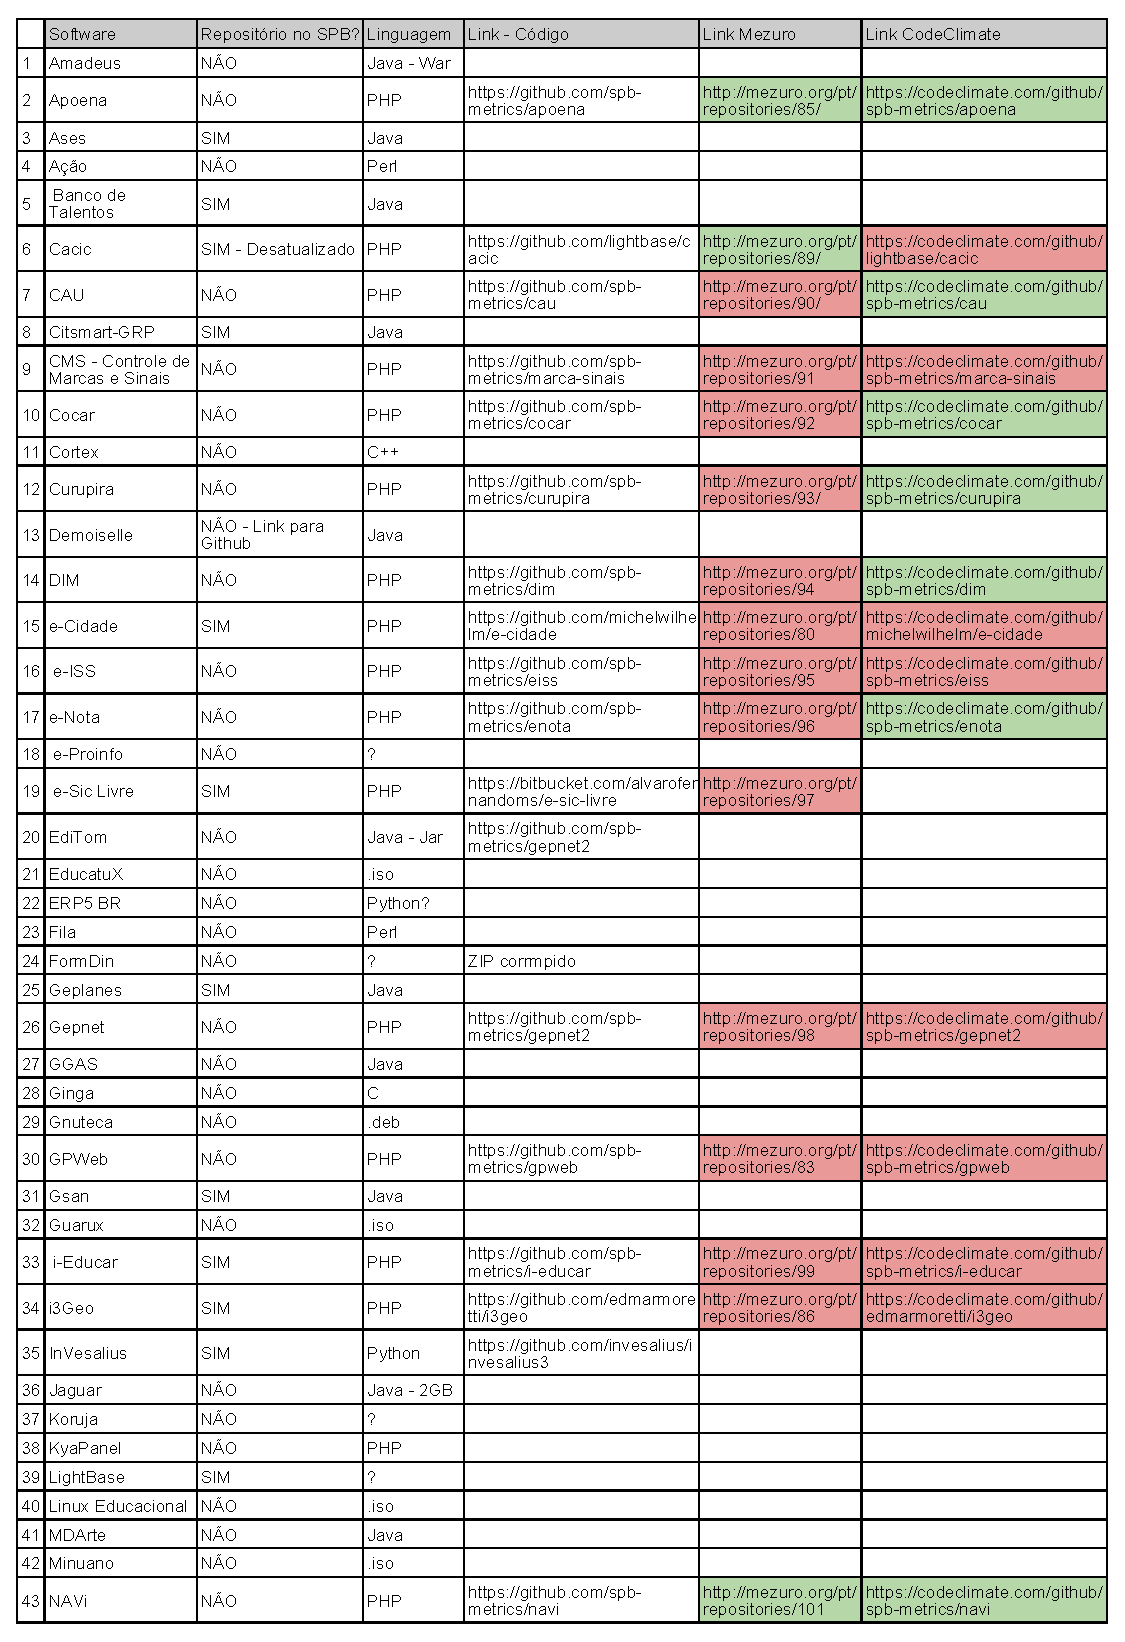
\includegraphics[keepaspectratio=true,scale=0.85]
    {tabelas/spb_1.eps}
  \caption{Categorização - Softwares SPB - Parte 1}
  \label{fig:softwares_spb_1}
\end{figure}

\begin{figure}[!htb]
	\centering
    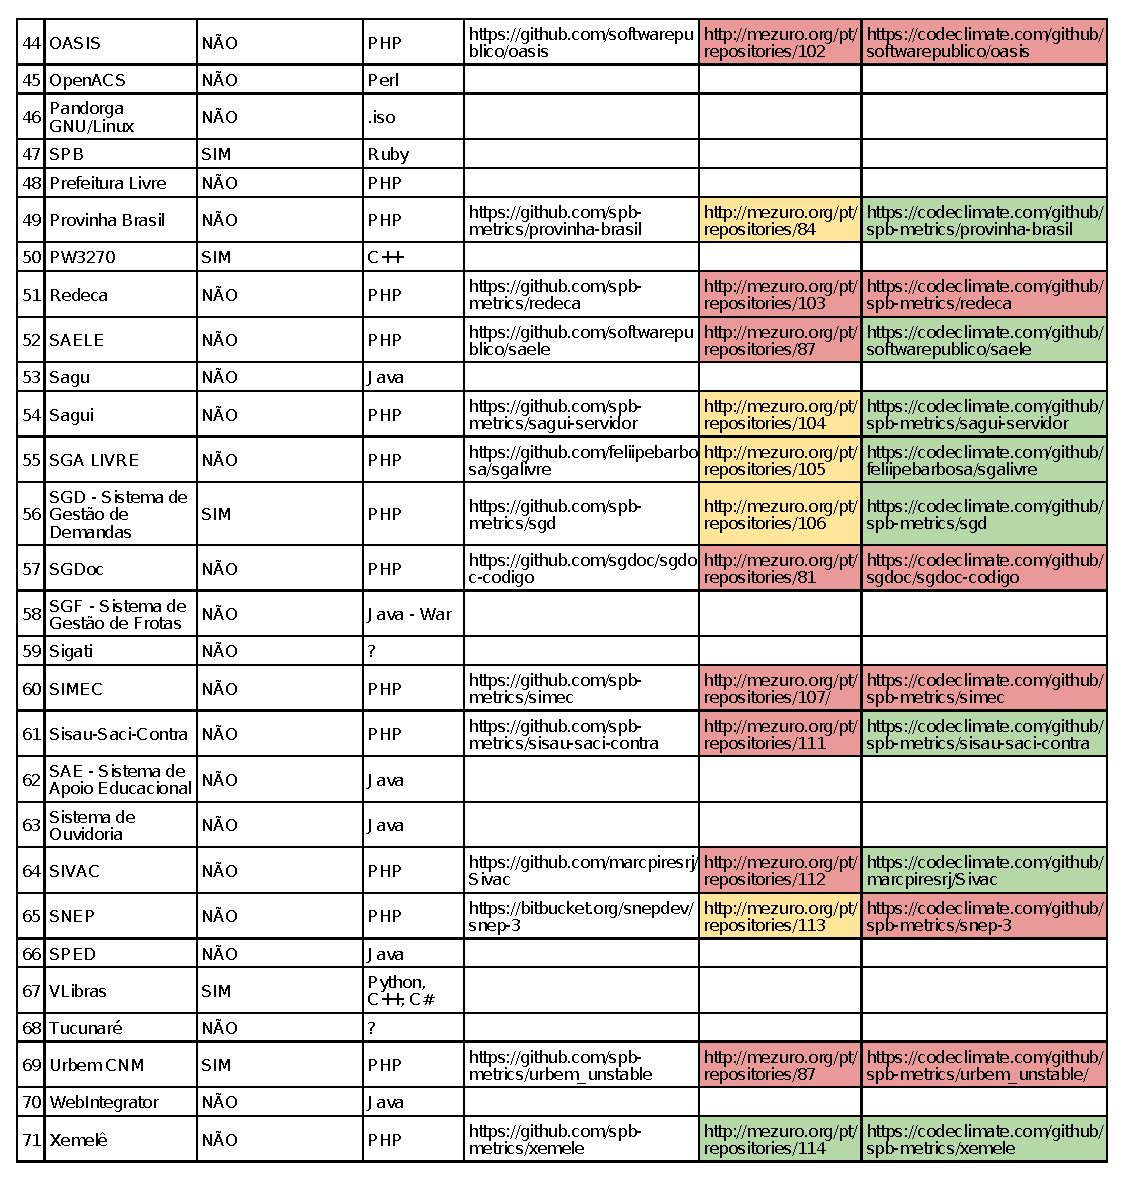
\includegraphics[keepaspectratio=true,scale=0.85]
    {tabelas/spb_2.eps}
  \caption{Categorização - Softwares SPB - Parte 2}
  \label{fig:softwares_spb_2}
\end{figure}

\end{anexosenv}

\printindex

\end{document}
